% !TEX root =../LibroTipoETSI.tex
\section{Estructura de \redborderddos}\label{sec:estructura}
\subsection{Configuración de red}\label{ssec:estructura_red}
Dado que uno de los estadísticos que \redborderddos{} debe controlar es la
relación entre el número de paquetes entrantes y salientes (como se vio en
la \ref{ssec:cusum_aplicado_trafico}), necesitamos una forma de distinguir el
sentido en el que el viaja el paquete. La forma escogida fue usar una interfaz
para los entrantes y otra interfaz distinta para los salientes, por lo que es
necesario, como mínimo, dos interfaces (+1 de gestión) para ejecutar
\redborderddos.

Desde el punto de vista de la arquitectura de red, \redborderddos{} debe colocarse en dos puertos SPAN\index{Puerto
SPAN} del conmutador que llegue al activo protegido, tal y como muestra la \autoref{fig:diagramaArquitectura}. Cada uno de los
puertos SPAN clonará los paquetes dirigidos hacia el activo a proteger, y los paquetes desde el activo a proteger
respectivamente, y los enviará hacia \redborderddos.
Si, además, se desea bloquear el tráfico, es necesario
un sistema que filtre las direcciones IP que se deben bloquear.
En ese momento es importante que el tráfico escaneado sea
previo al bloqueo, ya que de otra forma será imposible detectar el momento en el que el ataque ha sido detenido.

\begin{figure}[htbp]
\centering
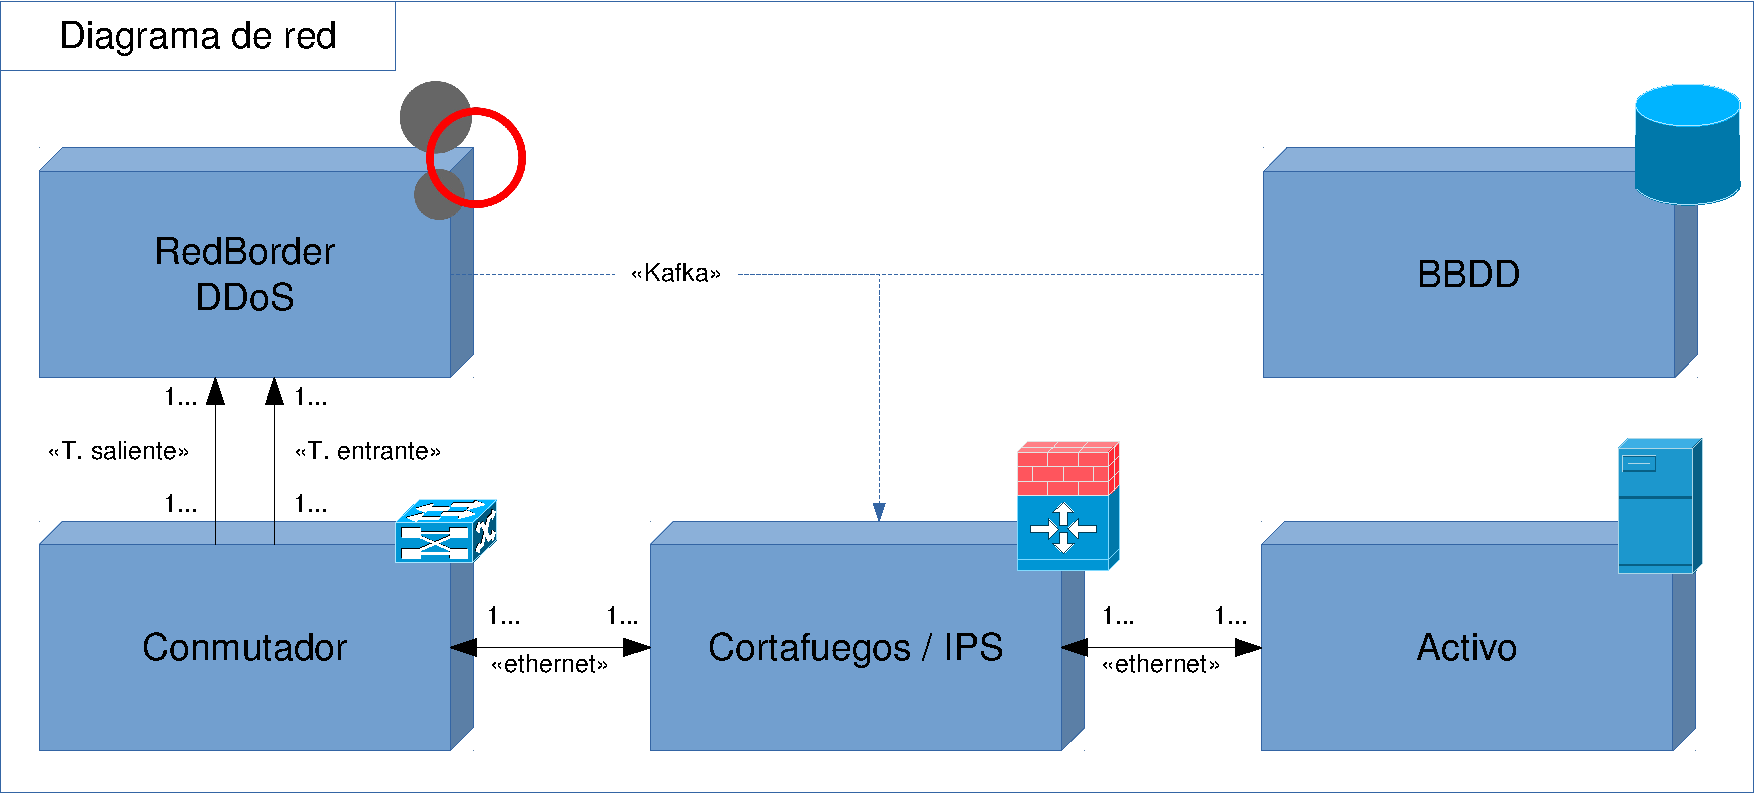
\includegraphics[width=\columnwidth]{CapituloEstructura/Figuras/DiagramaArquitectura-crop}
\caption{Diagrama de Arquitectura de \redborderddos}
\label{fig:diagramaArquitectura}
\end{figure}
%
%TODO Repasar las imágenes a fin de incluir el logotipo nuevo

Gracias al diseño modular de \redborderddos, es posible multiplexar los tráficos en los
que se recibe el tráfico entrante y saliente. Es decir, si el tráfico es muy elevado para
las interfaces, es posible usar más de un puerto para cualquiera de ellos, y, al mismo tiempo,
cualquier número de procesos para analizarlos.

\subsection{Uso de PF\_RING}
El sistema de captura del kernel de Linux es sistema ``de propósito general'', perfectamente capaz de
procesar paquetes a una tasa moderada para un uso común. Sin embargo,
algunas decisiones de diseño influyen muy negativamente en la tasa de captura\footnote{Al igual que,
por ejemplo, influye positivamente en la memoria usada por el mismo.}, y es necesario recurrir
a otras tecnologías para mejorar el caudal de captura.

PF\_RING es, según su autor Luca Deri, ``una tecnología que
persigue capturar tráfico a $10G$ sin necesitar tarjetas especializadas, sin pérdidas y bajo cualquier
circunstancia del tráfico, de forma que sea posible crear sondas de tráfico software con el mismo
rendimiento que las basadas en hardware'' \cite{LucaDeriPFRING}.

Con dicha tecnología, se prerreserva un anillo de memoria en exclusiva para la captura de paquetes,
evitando la sobrecarga que supone buscar bloques libres para almacenar los nuevos paquetes entrantes.
Es posible, además, que cualquier número de colas/aplicaciones acceda de manera concurrente y sin bloquear al mismo,
consiguiendo así la repartición $N$ tarjetas $\leftrightarrow$ $M$ procesadores explicada en
la \autoref{ssec:estructura_red}.

Por su parte, el uso de PF\_RING evita mucho procesamiento que normalmente hace el kernel, a la vez que evita
muchas copias internas. Si, además, se usa PF\_RING Zero-Copy se eliminan las copias y el paquete es leído
directamente de la tarjeta con lo que se hace posible leer los paquetes a la velocidad que llegan por
el cable -de cualquier tamaño- y usando tan sólo un hilo del procesador \cite{PFRingZc}. A partir de este momento,
podemos hablar de detectar ataques \gls{DoS} capturando los paquetes que lo provocan.

\subsection{Sistema de alerta}
Cuando un ataque se produce, \redborderddos{} es capaz de ser registrado en un fichero de texto
plano del disco duro y enviarlo por la plataforma Apache Kafka\index{Apache Kafka}.
Apache Kafka es un sistema
de ingesta de datos usado por la mayoría de bases de datos noSQL. En la 
alerta se registra la marca de tiempo del ataque, qué dirección IP ha ocasionado la alerta,
qué parámetros han sobrepasado sus valores límite y en qué magnitud.

\subsection{Estructura interna}
Internamente, \redborderddos{} se divide en los siguientes módulos, que se ven en la
\autoref{fig:diagramaActividad}.

\begin{figure}[htbp]
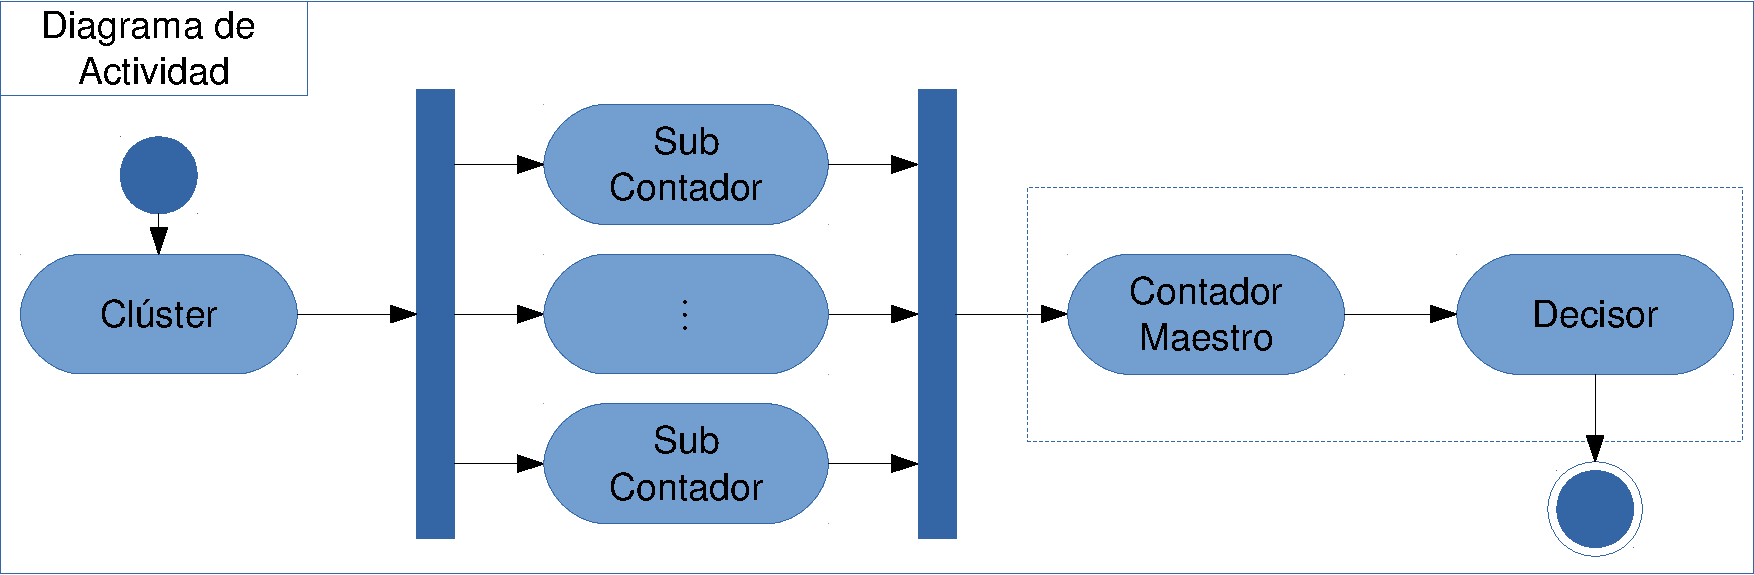
\includegraphics[width=\columnwidth]{CapituloEstructura/Figuras/DiagramaFlow-crop}
\caption{Diagrama de Actividad de \redborderddos}
\label{fig:diagramaActividad}
\end{figure}

El primer paso es el cluster, que al agrupar los paquetes entrantes y salientes de las distintas 
interfaces, indica el sentido de los mismos, y redirige los flujos (entendiendo flujo como aquellos
paquetes con las mismas direcciones de origen y destino así como sus respuestas) a los distintos 
sub-contadores de una forma coherente, haciendo que cada flujo llegue siempre a un mismo sub-contador.

Tras él, cada subcontador vigila los paquetes y bytes por cada protocolo, IP y el sentido
del tráfico, además de aquellos con las banderas \emph{SYN} y \emph{SYN+ACK}. A continuación,
el contador maestro aglutina periódicamente todos estos contadores y extrae los estadísticos
mencionados en la \autoref{ssec:cusum_aplicado_trafico}.

Internamente, cada subcontador almacena la información de cada flujo mediante una tabla hash,
a fin de agilizar la búsqueda de cada elemento. Cuando el contador maestro quiere comprobar
los estadísticos de un subcontador, el primero detiene al segundo y le arrebata su tabla hash,
entregándole una tabla limpia para que el subcontador pueda seguir realizando sus funciones. Al
mismo tiempo, los contadores ya están reservados en memoria, evitando así repetidas
llamadas a las funciones del sistema relacionadas con el manejo de memoria.

Con toda la piscina de contadores arrebatada, el contador maestro crea el conjunto de
estadísticos $x_i$ para cada flujo, y otro más para el contador general, y actualizará
el valor del CUSUM para cada uno. En el caso de que algún estadístico supere el umbral
establecido, se creará una alarma que se registrará en las salidas configuradas. Podemos
ver un ejemplo en \autoref{code:ejemplosAlarmaUmbral}, los bytes TCP recibidos estaban en
esa muestra a $\mu_0^{tcp\_bytes}+25\sigma^{tcp\_bytes}$, y sucesivos.

\begin{lstlisting}[language=json,caption={Ejemplo de alarma por umbral superado}, breaklines=true, 
label=code:ejemplosAlarmaUmbral,float=htbp,basicstyle=\scriptsize,captionpos=b]
{
 "timestamp": 1410602387, 
 "extern_ip": "8.8.8.8", 
 "positive_tcp_bytes_percent_value": 25.000,
 "negative_udp_bytes_percent_value": 6.667, 
 "positive_udp_pkts_percent_value": 13.333, 
 "reason": "threshold"
}
\end{lstlisting}

Por su parte, si detectamos una IP desconocida mientras estamos en el periodo de alerta,
se emitirá una alarma similar a la que se ve en \autoref{code:ejemplosAlarmaNuevaIP}.

\begin{lstlisting}[language=json,caption={Ejemplo de alarma por nueva IP}, breaklines=true, 
label=code:ejemplosAlarmaNuevaIP,float=htbp,captionpos=b,basicstyle=\scriptsize]
{
 "timestamp":1410622605,
 "extern_ip":"8.8.8.8",
 "reason":"New IP in alarm time"
}
\end{lstlisting}

\endinput
